\documentclass[aspectratio=169,11pt]{beamer}
\usepackage[T1]{fontenc}
\usepackage{lmodern,amsmath,amssymb,mathtools,bm,booktabs,array,graphicx,tikz}
\usetikzlibrary{arrows.meta,positioning,calc,decorations.pathreplacing,patterns}
\definecolor{ink}{HTML}{17344D}\definecolor{accent}{HTML}{087E8B}\definecolor{pale}{HTML}{EDF5F5}\definecolor{gold}{HTML}{AD6B19}
\providecommand{\dd}{\,\mathrm{d}}\providecommand{\R}{\mathbb{R}}
\providecommand{\E}{\mathbb{E}}\providecommand{\Var}{\operatorname{Var}}
\providecommand{\Cov}{\operatorname{Cov}}\providecommand{\diag}{\operatorname{diag}}
\providecommand{\norm}[1]{\left\lVert#1\right\rVert}
\providecommand{\abs}[1]{\left|#1\right|}
\usefonttheme{professionalfonts}
\setbeamercolor{normal text}{fg=black,bg=white}
\setbeamercolor{frametitle}{fg=ink,bg=white}
\setbeamercolor{title}{fg=ink}\setbeamercolor{structure}{fg=accent}
\setbeamercolor{block title}{fg=ink,bg=pale}\setbeamercolor{block body}{fg=black,bg=pale!40}
\setbeamercolor{alerted text}{fg=accent}
\setbeamerfont{frametitle}{size=\Large,series=\bfseries}
\setbeamerfont{title}{size=\LARGE,series=\bfseries}
\setbeamertemplate{navigation symbols}{}
\setbeamersize{text margin left=.7cm,text margin right=.7cm}
\setbeamertemplate{frametitle}{\vspace{.18cm}\insertframetitle\par\vspace{.1cm}{\color{accent}\hrule height .6pt}\vspace{.12cm}}
\newcommand{\notestarget}{notes.pdf}\newcommand{\noteslabel}{Notes}
\setbeamertemplate{footline}{\hspace{.7cm}\color{ink}\scriptsize Scientific Computing in Python\quad\href{\notestarget}{\noteslabel}\hfill\insertframenumber\,/\,\inserttotalframenumber\hspace{.7cm}\vspace{.18cm}}
\setbeamercovered{invisible}
\hypersetup{pdfauthor={Zan Ahmad},pdftitle={Python and sampled measurements},pdfpagemode=UseNone}
\begin{document}
\begin{frame}[plain]\vfill
{\small\color{accent} Scientific Computing in Python \quad Lecture 1}\par\medskip
{\raggedright\hyphenpenalty=10000\exhyphenpenalty=10000\LARGE\bfseries\color{ink} Python and sampled measurements}\par\bigskip
Zan Ahmad\par\smallskip
{\small Winter 2026}\par\vfill\end{frame}
\renewcommand{\notestarget}{notes.pdf\#note-values-and-assignment}
\begin{frame}[t,fragile,label=slide-values-and-assignment]{Values and assignment}
\begin{verbatim}
a = 4
b = 2*a
a = 7
\end{verbatim}
\pause{}
The final values are $a=7$ and $b=8$. The second line was evaluated before the third.
\end{frame}
\renewcommand{\notestarget}{notes.pdf\#note-values-and-assignment}
\begin{frame}[t,fragile,label=slide-expression-evaluation]{Expression evaluation}
\begin{verbatim}
x = 3
print(x**2 + 1)  # 10
print((x + 1)**2)  # 16
\end{verbatim}
\pause{}
Exponentiation uses \texttt{**}. Parentheses determine which quantity is squared.
\end{frame}
\renewcommand{\notestarget}{notes.pdf\#note-paired-observations}
\begin{frame}[t,fragile,label=slide-paired-observations]{Paired observations}
\[
(t_i,T_i)=(0,80),(60,62),(120,48),(180,38),(240,31).
\]
Time is in seconds and temperature in degrees Celsius.
\pause{}
\begin{verbatim}
time_seconds = [0, 60, 120, 180, 240]
temperature_c = [80, 62, 48, 38, 31]
\end{verbatim}
\end{frame}
\renewcommand{\notestarget}{notes.pdf\#note-paired-observations}
\begin{frame}[t,fragile,label=slide-indexing-the-endpoints]{Indexing the endpoints}
\begin{verbatim}
t0 = time_seconds[0]
t1 = time_seconds[-1]
T0 = temperature_c[0]
T1 = temperature_c[-1]
\end{verbatim}
\pause{}
The endpoint calculation uses $(0,80)$ and $(240,31)$. Interior observations remain relevant to the plotted record.
\end{frame}
\renewcommand{\notestarget}{notes.pdf\#note-units-and-affine-changes-of-scale}
\begin{frame}[t,fragile,label=slide-units-and-affine-changes-of-scale]{Units and affine changes of scale}
\[
t_{\rm min}=\frac{t_{\rm s}}{60},\qquad T_K=T_C+273.15.
\]
\pause{}
\[
\Delta T_K=(T_{C,1}+273.15)-(T_{C,0}+273.15)=\Delta T_C.
\]
\end{frame}
\renewcommand{\notestarget}{notes.pdf\#note-paired-observations}
\begin{frame}[label=slide-the-sampled-temperature-record-figure]{The sampled temperature record}
\centering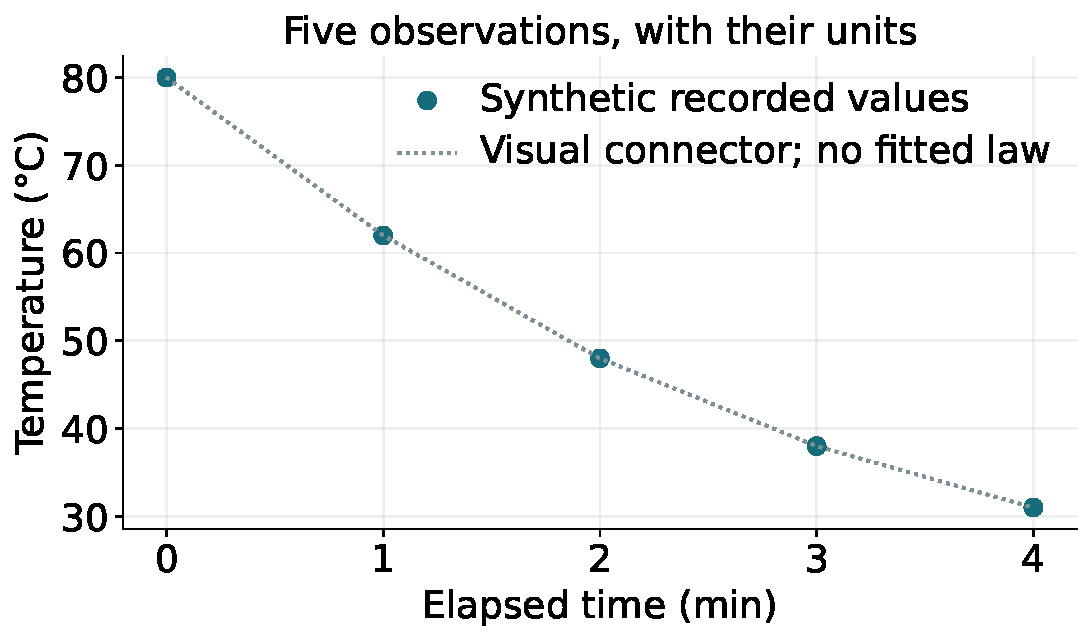
\includegraphics[width=.98\linewidth,height=.69\textheight,keepaspectratio]{presentation-figures/temperature-record.pdf}\end{frame}
\renewcommand{\notestarget}{notes.pdf\#note-units-and-affine-changes-of-scale}
\begin{frame}[t,fragile,label=slide-the-same-change-in-two-units]{The same change in two units}
\[
\Delta T=31-80=-49\ ^\circ\mathrm C=-49\ \mathrm K.
\]
\pause{}
\[
\Delta t=240\ \mathrm s=4\ \mathrm{min}.
\]
Temperature differences have equal numerical values in Celsius and kelvin. Absolute temperatures do not.
\end{frame}
\renewcommand{\notestarget}{notes.pdf\#note-average-rate-of-change}
\begin{frame}[t,fragile,label=slide-average-rate-of-change]{Average rate of change}
\[
\overline r=\frac{T_1-T_0}{t_1-t_0},\qquad t_1>t_0.
\]
\pause{}
\[
\overline r=\frac{-49}{4}=-12.25\ ^\circ\mathrm C/\mathrm{min}.
\]
This is an interval average, not an instantaneous derivative.
\end{frame}
\renewcommand{\notestarget}{notes.pdf\#note-average-rate-of-change}
\begin{frame}[t,fragile,label=slide-a-direct-python-calculation]{A direct Python calculation}
\begin{verbatim}
elapsed_min = (time_seconds[-1]-time_seconds[0])/60
change_c = temperature_c[-1]-temperature_c[0]
rate_c_per_min = change_c/elapsed_min
\end{verbatim}
\pause{}
A zero elapsed time would make the quotient undefined. The denominator must be checked before division.
\end{frame}
\renewcommand{\notestarget}{notes.pdf\#note-floating-point-arithmetic}
\begin{frame}[t,fragile,label=slide-floating-point-arithmetic]{Floating-point arithmetic}
\begin{verbatim}
0.1 + 0.2 == 0.3  # False in binary floating point
\end{verbatim}
\pause{}
A useful comparison has the form
\[
|a-b|\leq \varepsilon_{\rm abs}+\varepsilon_{\rm rel}|b|.
\]
\end{frame}
\renewcommand{\notestarget}{notes.pdf\#note-units-and-affine-changes-of-scale}
\begin{frame}[label=slide-celsius-and-kelvin-figure]{Celsius and kelvin}
\centering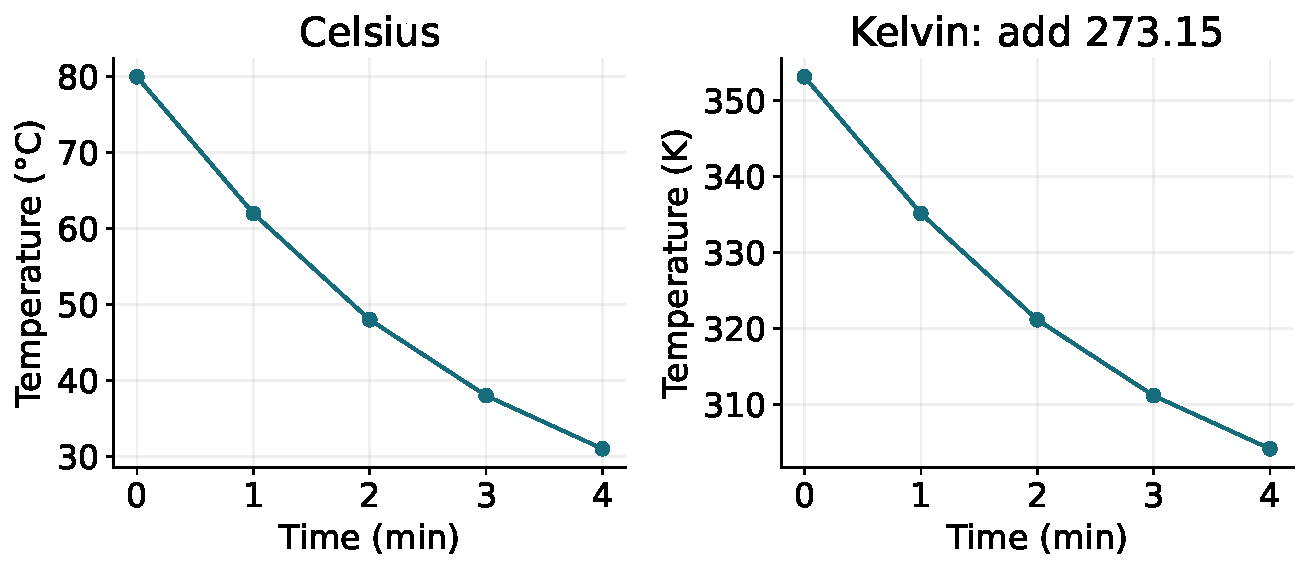
\includegraphics[width=.98\linewidth,height=.69\textheight,keepaspectratio]{temperature-scales.pdf}\end{frame}
\renewcommand{\notestarget}{notes.pdf\#note-floating-point-arithmetic}
\begin{frame}[t,fragile,label=slide-scale-in-an-error-tolerance]{Scale in an error tolerance}
The absolute term controls comparisons near zero. The relative term scales with the reference magnitude.
\pause{}
\[
|60r_{\rm s}-r_{\rm min}|\leq 10^{-12}
\]
is a numerical unit-conversion check for this small example. It is not a statement about thermometer accuracy.
\end{frame}
\renewcommand{\notestarget}{notes.pdf\#note-plots-and-reproducible-execution}
\begin{frame}[t,fragile,label=slide-plots-and-reproducible-execution]{Plots and reproducible execution}
Five observations determine five plotted points. They do not determine the complete function $T(t)$.
\pause{}
If $g(t_i)=0$ at every sampled time, both $T(t)$ and $T(t)+g(t)$ fit those observations.
\end{frame}
\renewcommand{\notestarget}{notes.pdf\#note-plots-and-reproducible-execution}
\begin{frame}[t,fragile,label=slide-a-family-of-indistinguishable-interpolants]{A family of indistinguishable interpolants}
For any constant $c$,
\[
g(t)=c\prod_{i=0}^{4}(t-t_i)
\]
vanishes at all five sample times.
\pause{}
Additional assumptions are required to infer behavior between observations.
\end{frame}
\end{document}
